\documentclass[border=4pt]{standalone}
\usepackage{fontspec}
\usepackage{amsmath}
\usepackage{unicode-math}
\setmainfont{Latin Modern Roman}
\setmathfont{Latin Modern Math}
\usepackage{pgfplots}
\usepackage{pgfplotstable}
\pgfplotsset{compat=1.18}
\usepackage{tkz-euclide}
\usetikzlibrary{arrows.meta,calc,angles,quotes,patterns,3d,backgrounds}
\definecolor{ink}{HTML}{123428}
\definecolor{asy}{HTML}{475569}
\definecolor{mint}{HTML}{86e0bd}
\tikzset{asym/.style={asy, line width=0.9pt, dash pattern=on 5pt off 3.5pt},
         guide/.style={gray!70, line width=0.6pt, densely dotted},
         dot/.style={circle, inner sep=0pt, minimum size=5pt, draw=white, line width=0.5pt},
         odot/.style={circle, inner sep=0pt, minimum size=5.5pt, fill=white, line width=1pt},
         lab/.style={font=\footnotesize, inner sep=1.5pt, text=ink}}
\begin{document}
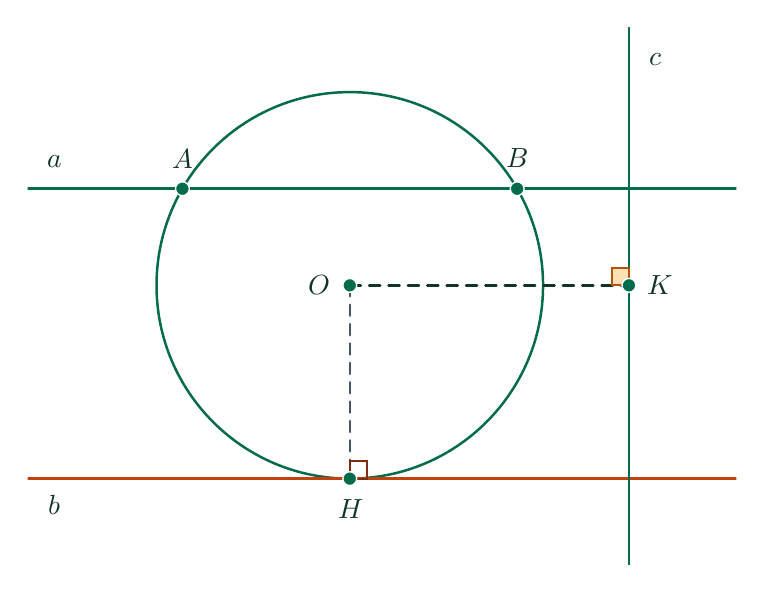
\begin{tikzpicture}[x=1.3636cm, y=1.3636cm]
\tkzDefPoint(0,0){O}
\tkzDefPoint(-1.5588,0.9){A}
\tkzDefPoint(1.5588,0.9){B}
\tkzDefPoint(0,-1.8){H}
\tkzDefPoint(2.6,0){K}
\tkzDefPoint(2.6,1){K2}
\tkzDefPoint(1.8,0){tmp1}
\tkzDefPoint(-3,0.9){tmp2}
\tkzDefPoint(3.6,0.9){tmp3}
\tkzDefPoint(-3,-1.8){tmp4}
\tkzDefPoint(3.6,-1.8){tmp5}
\tkzDefPoint(3.6,-1.8){tmp6}
\tkzDefPoint(2.6,2.4){tmp7}
\tkzDefPoint(2.6,-2.6){tmp8}
\begin{scope}
\clip (-3.0,-2.6) rectangle (3.6,2.4);
\tkzDrawCircle[draw={rgb,255:red,4;green,107;blue,77}, line width=0.9pt](O,tmp1)
\tkzDrawSegment[draw={rgb,255:red,4;green,107;blue,77}, line width=0.90pt](tmp2,tmp3)
\tkzDrawSegment[draw={rgb,255:red,71;green,85;blue,105}, line width=0.90pt, dash pattern=on 4pt off 3pt](O,H)
\tkzDrawSegment[draw={rgb,255:red,194;green,65;blue,12}, line width=1.08pt](tmp4,tmp5)
\tkzDrawSegment[draw={rgb,255:red,4;green,107;blue,77}, line width=0.90pt](tmp7,tmp8)
\tkzDrawSegment[draw=ink, line width=0.90pt, dash pattern=on 4pt off 3pt](O,K)
\end{scope}
\tkzMarkRightAngle[size=0.22, draw={rgb,255:red,124;green,45;blue,18}, line width=0.7pt](O,H,tmp6)
\tkzMarkRightAngle[size=0.22, draw={rgb,255:red,180;green,83;blue,9}, line width=0.7pt, fill={rgb,255:red,245;green,158;blue,11}, fill opacity=0.3](K2,K,O)
\node[dot, fill={rgb,255:red,4;green,107;blue,77}] at (O) {};
\node[dot, fill={rgb,255:red,4;green,107;blue,77}] at (A) {};
\node[dot, fill={rgb,255:red,4;green,107;blue,77}] at (B) {};
\node[dot, fill={rgb,255:red,4;green,107;blue,77}] at (H) {};
\node[dot, fill={rgb,255:red,4;green,107;blue,77}] at (K) {};
\node[lab, font=\normalsize] at (-2.75,1.15) {$a$};
\node[lab, font=\normalsize] at (-2.75,-2.05) {$b$};
\node[lab, font=\normalsize] at (2.85,2.1) {$c$};
\node[lab, font=\normalsize, anchor=center, xshift=-11pt, yshift=0pt] at (0,0) {$O$};
\node[lab, font=\normalsize, anchor=center, xshift=0pt, yshift=11pt] at (-1.5588,0.9) {$A$};
\node[lab, font=\normalsize, anchor=center, xshift=0pt, yshift=11pt] at (1.5588,0.9) {$B$};
\node[lab, font=\normalsize, anchor=center, xshift=0pt, yshift=-11pt] at (0,-1.8) {$H$};
\node[lab, font=\normalsize, anchor=center, xshift=11pt, yshift=0pt] at (2.6,0) {$K$};
\end{tikzpicture}
\end{document}
